\documentclass[a4paper]{article}

\usepackage[english]{babel}
\usepackage{amsmath}
\usepackage{amssymb}
\usepackage{dsfont}
\usepackage{tikz}
\usepackage{framed} 
\usetikzlibrary{arrows,automata}
\title{Calculus and Probability Theory\\ Assignment 4}
\author{Christoph Schmidl\\
s4226887\\
Data Science\\
c.schmidl@student.ru.nl\\}
\date{\today}


\begin{document}
\maketitle





\textbf{After completing these exercises successfully you should be confident with the following topics:}

\begin{itemize}
	\item Analyse and sketch real functions
	\item Apply differentiation rules to determine higher-order partial derivatives
	\item Find primitives of well-known functions
	\item Compute definite integrals when the primitive function is known
	\item computer improper integrals
\end{itemize}
\vspace{1em}

\begin{enumerate}


%%%%%%%%%%%% Task 1 %%%%%%%%%%%%
\item (\textbf{20 points}) Investigate the function $f(x) = \frac{x}{\ln(x)}$ as follows. (Do not start with drawing a graph by means of a device or some web resource. Of couse you may check your result when you're done.)

\begin{enumerate}
	%%%%%%%% Task 1.a %%%%%%%%
	\item Determine the domain of the function $f$.\\
	\textbf{Solutions:}\\
	
In this case, we just have to look out for the values for x when the denominator could become 0 or undefined. First of all, $\ln(0)$ is undefined. Second, $\ln(1) = 0$. Note for myself: $\ln(1) = 0$ answers the question, what is the value for x so $e^x = 1$?. Therefore:	
	
	\begin{equation}
		D(f) = \{ x \in \mathbb{R} \; | \;  0 < x < 1 \wedge x > 1\} \notag
	\end{equation}
	
	
	%%%%%%%% Task 1.b %%%%%%%%
	\item What are the roots of $f$?\\
	\textbf{Solutions:}\\

To determine the roots of f, we just have to determine the x value when the whole quotient equals 0. As we take the denominator as the first step, then we plug in x = 0 and get $\ln(0) = 1$ and in the numerator 0. Therefore $\frac{0}{\ln(0)} = \frac{0}{1} = 0$.\\

The roots of f: $x_1 = 0$\\

The y-intercept would therefore also be 0.\\



	%%%%%%%% Task 1.c %%%%%%%%
	\item Determine the limits at 1 and $\infty$. (Hint: there are 3 cases, use L'Hopital!)\\
	\textbf{Solutions:}\\
	

	\begin{align*}
		\lim_{x \to 1^-} \frac{x}{\ln(x)} &= \lim_{x \to 1^-} \frac{1}{\frac{1}{x}}\\
		&= \lim_{x \to 1^-} \frac{1}{\frac{1}{x}}\\
		&= \lim_{x \to 1^-} x\\
		&= -\infty
	\end{align*}
	
		\begin{align*}
		\lim_{x \to 1^+} \frac{x}{\ln(x)} &= \lim_{x \to 1^+} \frac{1}{\frac{1}{x}}\\
		&= \lim_{x \to 1^+} \frac{1}{\frac{1}{x}}\\
		&= \lim_{x \to 1^+} x\\
		&= \infty
	\end{align*}
	
			\begin{align*}
		\lim_{x \to \infty} \frac{x}{\ln(x)} &= \lim_{x \to \infty} \frac{1}{\frac{1}{x}}\\
		&= \lim_{x \to \infty} \frac{1}{\frac{1}{x}}\\
		&= \lim_{x \to \infty} x\\
		&= \infty
	\end{align*}


	%%%%%%%% Task 1.d %%%%%%%%
	\item Find $f'$ and $f''$.\\
	\textbf{Solutions:}\\

Use Quotient rule.

	\begin{align*}
		f(x)' &= \frac{1 \cdot ln(x) - x \cdot \frac{1}{x}}{ln^2(x)}\\
		&= \frac{\ln(x) - 1}{\ln^2(x)}\\
	\end{align*}
	
	\begin{align*}
		f(x)'' &= \frac{\frac{1}{x} \ln^2(x) - ((\ln(x) - 1) \frac{2\ln(x)}{x})}{ln^4(x)}\\
		&= \frac{\frac{\ln^2(x) - ((\ln(x) - 1)2\ln(x))}{x}}{\ln^4(x)}\\
		&= \frac{\frac{\ln(x) - (2\ln(x) - 2)}{x}}{\ln^3(x)}\\
		&= \frac{\frac{-\ln(x) + 2}{x}}{\ln^3(x)}\\
		&= \frac{2 - \ln(x)}{x \ln^3(x)}
	\end{align*}


	
	%%%%%%%% Task 1.e %%%%%%%%
	\item Find the zeros of $f'$ and $f''$.\\
	\textbf{Solutions:}\\
	
$f'(x) = \frac{ln(x) - 1}{ln^2(x)}$ so $x = e$ is the only zero of $f'(x)$.\\
$f''(x) = \frac{2 - \ln(x)}{x \ln^3(x)}$ so $x = e^2$ is the only zero of $f''(x)$.\\		
	
	
	
	%%%%%%%% Task 1.f %%%%%%%%
	\item What are the critical points (determine their $x$ and $y$ coordinates)?\\
	\textbf{Solutions:}\\
	
A critical point of a function $f: D \rightarrow \mathbb{R}$, is a point $a \in D$ such that $f'(a) = 0$. The value $f(a)$ is called a critical value of f.\\

We just found the x-coordinates of the critical point. We have $f(e) = \frac{e}{ln(e)} = \frac{e}{1} = 1$. So we get the point (e,e).\\



	
	
	
	
	%%%%%%%% Task 1.g %%%%%%%%
	\item Find the local minimums and maximums.\\
	\textbf{Solutions:}\\
	
We have $f''(e) = \frac{2 - ln(e)}{x \ln^3(e)} = \frac{2 - 1}{e \cdot 1} = \frac{1}{e} > 0$, so it is a minimum. This is the only critical point, so there are no local maxima and only one minimum.\\	
	
	
	
	%%%%%%%% Task 1.h %%%%%%%%
	\item Which parts of the function are convex and concave? Does function $f$ have points of inflection? (Hint: Use the sign of the second derivative for answering both questions.)\\
	\textbf{Solutions:}\\
	
	The function is concave $\Longleftrightarrow f''(x) < 0 \Longleftrightarrow \frac{2 -  \ln(x)}{x \ln^3(x)} < 0 \Longleftrightarrow x < e^2$.\\
	The function is convex $\Longleftrightarrow f''(x) > 0 \Longleftrightarrow \frac{2 -  \ln(x)}{x \ln^3(x)} > 0 \Longleftrightarrow x > e^2$.\\
	It has a point of inflection at $x = e^2$\\
	
	%%%%%%%% Task 1.i %%%%%%%%
	\item Draw the graph of function $f$. (If you collect all intervals and special points in a table, it helps a lot in drawing the graph. Moreover, you get some extra points!)\\
	\textbf{Solutions:}\\	
	
	
	\begin{figure}[ht!]
	\centering
  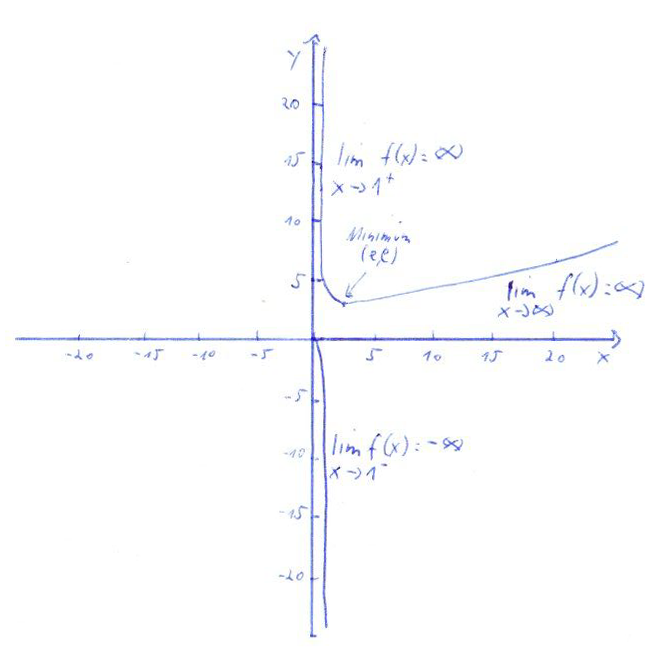
\includegraphics[width=0.7\textwidth]{images/1i.PNG}
\end{figure}		
	
	
\end{enumerate}


%%%%%%%%%%%% Task 2 %%%%%%%%%%%%
\item (\textbf{6 points}) Show that the derivative of an odd function is even and that the derivative of an even function is odd.\\
\textbf{Solutions:}\

\begin{itemize}
	\item A function $f : (-a,a) \rightarrow \mathbb{R}$ is even if $f(-x) = f(x)$, for all $x \in (a-,a)$ and odd if $f(-x) = -f(x)$, for all $x \in (-a,a)$
	\item $f'(x) = \lim_{h \to 0} \frac{f(x + h) - f(x)}{h}$
\end{itemize}

If $f$ is odd then

\begin{align*}
	f'(-x) = \lim_{h \to 0} \frac{f(-x + h) - f(-x)}{h} = - \lim_{h \to 0} \frac{f(x - h) - f(x)}{h} = - f'(x)
\end{align*}


%%%%%%%%%%%% Task 3 %%%%%%%%%%%%
\item (\textbf{14 points}) Optimization problem 

\begin{enumerate}
	%%%%%%%% Task 3.a %%%%%%%%
	\item Find the point on the parabola $y^2 = 2x$ that is closest to $A = (1,4)$\\
	\textbf{Solutions:}\\
	
$y^2 = 2x$ is a sideways parabola with the equation $x = \frac{y^2}{2}$.\\
The distance formula from unknown point (x,y) to known point A = (1,4) is

\begin{align*}
	d(x,y) = \sqrt{(x-1)^2 + (y - 4)^2} \notag
\end{align*}	

Substitute $\frac{y^2}{2}$ for x:

\begin{align*}
d(\frac{y^2}{2},y) &= \sqrt{(\frac{y^2}{2} - 1) + (y - 4)^2}\\
d(y) &= \sqrt{\frac{y^4}{4} - y^2 + 1 + 2 - 8y + 16}\\
&= \sqrt{\frac{y^4}{4} - 8y + 17}
\end{align*}	

Take the derivative of the distance with respect to y

\begin{align*}
d'(y) = \frac{y^3 - 8}{\sqrt{y^4 - 32y + 68}}
\end{align*}

The minimum will occur when the derivative is zero:

\begin{align*}
	y^3 - 8 &= 0\\
	y^3 &= 8 \\
	y &= 2\\
	x &= \frac{2^2}{2}\\
	x &= 2
\end{align*}

The point (2,2) is the closest point on the parabola to A = (1,4).\\	
	
	%%%%%%%% Task 3.b %%%%%%%%
	\item A steel rod is carried down a hallway of 9 meter wide. At the end there is a corner to the right into a narrower hallway of 6 meter wide. What is the maximum length of the steel rod that can be carried horizontally around the corner?
	
	\begin{figure}[ht!]
	\centering
  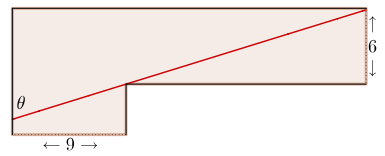
\includegraphics[width=0.7\textwidth]{images/task3.PNG}
\end{figure}	
	
	
	(Hint: What happens at $\theta \rightarrow 0$ and $\theta \rightarrow \frac{1}{4} \pi$? Show that the angle at which the minimum is obtained is at $\theta = arctan(\sqrt[3]{\frac{3}{2}}) \approx 0,853$.)
	\textbf{Solutions:}\\	
	
		
\end{enumerate}





%%%%%%%%%%%% Task 4 %%%%%%%%%%%%
\item (\textbf{20 points}) Given function $f$, find the partial derivatives. If it is necessary, simplify the result.

\begin{enumerate}
	%%%%%%%% Task 4.a.i %%%%%%%%
	\item[a.i] $f(x,y) = \cos(4y - xy)$; $\frac{\partial}{\partial x}f(x,y) = ?$\\
	\textbf{Solutions:}
	
	\begin{align}
		\frac{\partial}{\partial x}f(x,y) &= -sin(4y - xy)(-y)\notag\\
		&= y \sin(4y-xy) \notag
	\end{align}
	

	\item[a.ii] $f(x,y) = \cos(4y - xy)$; $\frac{\partial}{\partial y}f(x,y) = ?$\\\
	\textbf{Solutions:}
	
		\begin{align}
		\frac{\partial}{\partial y}f(x,y) &= -sin(4y-xy)(4-x)\notag\\
		&= (x-4)sin(4y - xy)\notag
	\end{align}
	\vspace{1em}
		
		
	%%%%%%%% Task 4.b %%%%%%%%%
	\item[b] Show that $\frac{\partial}{\partial x}(\frac{\partial}{\partial y}f(x,y)) = \frac{\partial}{\partial y}(\frac{\partial}{\partial x}f(x,y))$\\
	\textbf{Solutions:}		
		
The \textbf{Theorem of Schwarz} says that it does not matter in which order you take two partial derivatives:

\begin{align*}
	\frac{\partial^2 f}{\partial x \partial y} = \frac{\partial^2 f}{\partial y \partial x}
\end{align*}	
	
	
		
If we differentiate $f$ first with respect to $x$ and then with respect to $y$ we get the derivative $\frac{\partial}{\partial y} (\frac{\partial f}{\partial x})$ (if it exists). It is more usually denoted by $\frac{\partial^2 f}{\partial y \partial x}$ or $(f_x')_y'$ or $f_{xy}''$\\

Alternatively, if we differentiate first with respect to $y$ and then $x$ we get $\frac{\partial}{\partial x} (\frac{\partial f}{\partial y}) = \frac{\partial^2 f}{\partial x \partial y}$ (if it exists). Or $(f_y')_x'$ or $f_{yx}''$
		
Let's rewrite the left-hand side of the formula	$\frac{\partial}{\partial x}(\frac{\partial}{\partial y}f(x,y)) = \frac{\partial}{\partial y}(\frac{\partial}{\partial x}f(x,y))$ like this:

\begin{align*}
	\frac{\partial}{\partial x}(\frac{\partial}{\partial y}f(x,y)) &= \frac{\partial}{\partial x}(\lim_{h \to 0} \frac{f(x + h,y) - f(x,y)}{h})%
\end{align*}
		
		
		
\end{enumerate}




%%%%%%%%%%%% Task 5 %%%%%%%%%%%%
\item (\textbf{20 points}) Evaluate the following definite integrals. (Hint: use slide 38 of the lectures about derivatives, and slide 13 of the lectures about primitives)

\begin{align}
	\int_{a}^b f(x) dx = F(b) - F(a)\notag
\end{align}



\begin{enumerate}
	%%%%%%%% Task 5.a %%%%%%%%
	\item $\int_{-1}^1(x^3 + x - 1)dx$\\
	
	\textbf{Solutions:}
	
\begin{align}
	\int (x^3 + x - 1)dx &= \frac{1}{4}x^4 + \frac{1}{2}x^2 - x + C \notag\\
	\int_{-1}^1(x^3 + x - 1)dx &= \left[ \frac{1}{4}1^4 + \frac{1}{2}1^2 - 1  \right] - \left[ \frac{1}{4}(-1)^4 + \frac{1}{2}(-1)^2 - (-1)\right]\notag\\
	&= \frac{1}{4} - \frac{1}{2} - \frac{1}{4} - \frac{1}{2} - 1\notag\\
	&= -2\notag
\end{align}	
	
	
	%%%%%%%% Task 5.b %%%%%%%%
	\item $\int_{1}^2(3\sqrt{x} + \frac{3}{x^2})dx$\\
	
	\textbf{Solutions:}
	
\begin{align}
	\int(3\sqrt{x} + \frac{3}{x^2})dx &= 3 \left[ \frac{2x^\frac{3}{2}}{3} - \frac{1}{x}\right] + C\notag\\
	\int_{1}^2(3\sqrt{x} + \frac{3}{x^2})dx &= \left[ 3(\frac{2(2)^\frac{3}{2}}{3} - \frac{1}{2})\right] - \left[ 3(\frac{2(1)^\frac{3}{2}}{3} - 1) \right]\notag\\
	&= 4\sqrt{2} - \frac{1}{2}\notag\\
	&\approx 5.1569\notag
\end{align}		
	
	
	%%%%%%%% Task 5.c %%%%%%%%
	\item $\int_{0}^\pi(\sin(x) + \cos(x))dx$\\
	
	\textbf{Solutions:}	

\begin{align}
	\int(\sin(x) + \cos(x))dx &= -\cos(x) + \sin(x) + C\notag\\
	\int_{0}^\pi(\sin(x) + \cos(x))dx &= \left[ -\cos(\pi) + \sin(\pi))\right] - \left[ -\cos(0) + \sin(0)\right]\notag\\
	&= 1 + 0 + 1 + 0\notag\\
	&= 2\notag
\end{align}		




	%%%%%%%% Task 5.d %%%%%%%%
	\item $\int_{1}^e(\frac{1 - \ln x}{x^2})dx$\\
	
	\textbf{Solutions:}	

Integration by parts:

\begin{align}
	\int(\frac{1 - \ln x}{x^2})dx &=  \int((1 - \ln x)\frac{1}{x^2})dx = \int((1 - \ln x)x^{-2})dx \notag\\
	&= \left[ (1 - ln x) (-\frac{1}{x})\right] - \int -\frac{1}{x} (-\frac{1}{x})\notag\\
	&= \left[ (1 - ln x) (-\frac{1}{x})\right] - \int \frac{1}{x^2}\notag\\
	&= \left[ (1 - ln x) (-\frac{1}{x})\right] + \frac{1}{x}\notag\\
	&= \frac{ln x}{x}\notag\\
	\int_{1}^e(\frac{1 - \ln x}{x^2})dx &= \frac{ln(e)}{e} - \frac{ln(1)}{1}\notag\\
	&= \frac{1}{e} - \frac{0}{1}\notag\\
	&= \frac{1}{e}\notag
\end{align}		



\end{enumerate}


%%%%%%%%%%%% Task 6 %%%%%%%%%%%%
\item (\textbf{20 points}) Evaluate the following improper integrals.

\begin{enumerate}
	%%%%%%%% Task 6.a %%%%%%%%
	\item $\int_{-1}^1 (\frac{1}{x^n})dx$, $n$ an integer such that $n \geq 2$; (Hint: distinguish two cases).\\
	\textbf{Solutions:}	
	
	
	
	
	%%%%%%%% Task 6.b %%%%%%%%
	\item $\int_{-\infty}^{-\pi/2}\frac{x \cos(x) - \sin(x)}{x^2}dx$; (Hint: use the quotient rule for derivation to find the primitive)\\
	\textbf{Solutions:}	

\begin{align}
	\int(\frac{x \cos(x) - \sin(x)}{x^2})dx &= \frac{\sin(x)}{x} + C\notag\\
	\int_{-\infty}^{-\pi/2}(\frac{x \cos(x) - \sin(x)}{x^2})dx &= \frac{2}{\pi}\notag
\end{align}	


	%%%%%%%% Task 6.c %%%%%%%%
	\item $\int_{2}^{\infty}\frac{-1}{x \ln^2(x)} dx$; (Hint: use a fraction of well known functions to find the primitive)\\
	\textbf{Solutions:}	
	
\begin{align}
	\int(\frac{-1}{x \ln^2(x)})dx &= \frac{1}{\ln(x)} + C\notag\\
\int_{2}^{\infty}(\frac{-1}{x \ln^2(x)}) dx &= \frac{1}{\ln(2)}\notag
\end{align}	


\end{enumerate}


%%%%%%%%%%%% Task 7 %%%%%%%%%%%%
\item (\textbf{bonus, +6 points}) Find primitves of the following functions $f$. That is, find $F$ such that $F'(x) = f(x)$.

\begin{enumerate}
	%%%%%%%% Task 8.a %%%%%%%%
	\item $f(x) = \frac{1}{2 \sqrt{x}} - \frac{1}{x^2}$\\
	\textbf{Solutions:}		
	
\begin{align}
	\int(\frac{1}{2 \sqrt{x}} - \frac{1}{x^2})dx &= \sqrt{x} + \frac{1}{x} + C\notag
\end{align}		
	
	
	
	
	%%%%%%%% Task 7.b %%%%%%%%
	\item $f(x) = 2 \sin(x) \cos(x)$\\
	\textbf{Solutions:}	
	
Integration by parts:	
	
\begin{align}
	\int(2 \sin(x) \cos(x))dx &= - \frac{1}{2} \cos(2x) + C\notag
\end{align}		
	
	
	%%%%%%%% Task 7.c %%%%%%%%
	\item $f(x) = \frac{2}{1 + 4x^2}$\\
	\textbf{Solutions:}		
	
Integration by parts:	
	
\begin{align}
	\int(\frac{2}{1 + 4x^2})dx &= \arctan(2x) + C\notag
\end{align}					
	

\end{enumerate}

%%%%%%%%%%%% Task 8 %%%%%%%%%%%%
\item (\textbf{bonus, 10 points}) If $f(x,y) = \frac{xy}{x+y}$, show that

\begin{align}
x^2 \cdot \frac{\partial}{\partial x}(\frac{\partial}{\partial x}f(x,y)) + 2xy \cdot \frac{\partial}{\partial x}(\frac{\partial}{\partial y}f(x,y)) + y^2 \cdot \frac{\partial}{\partial y}(\frac{\partial}{\partial y}f(x,y)) = 0\notag
\end{align}
	(Hint: First compute all the second partial derivatives of $f$, then substitute the results in the expression on the left-hand side.)\\
\textbf{Solutions:}	

\end{enumerate}

\end{document}
